
\chapter{Theoretical description of quantum jumps\label{chap:theoretical-description-jumps} }

\addcontentsline{lof}{chapter}{Theoretical description of quantum jumps\lofpost}  
%\addcontentsline{lot}{chapter}{Theoretical description of quantum jumps\lofpost}

\singlespacing 
\setlength{\epigraphwidth}{.6\textwidth}
\epigraph{
Photons, the quanta of light, are countable and discrete, and one assumes they come and go in jumps. Einstein proposed it so --- though only as a pragmatic step  ... Yet the Schrödinger equation is deterministic and nothing within its jurisdiction jumps. What then to make of this unlikely marriage where the continuous is to somehow cavort with the discrete.}
{H.J. Carmichael\\New Zealand Science Review\\ Vol. 72 (2) 2015} 
\setlength{\epigraphwidth}{.4\textwidth} % default
\doublespacing\noindent\lettrine{T}{his} chapter presents the quantum trajectory
description of the Dehmelt electron-shelving scheme and the catch-and-reverse
circuit quantum electrodynamics (cQED) experiment. Section~\ref{sec:Fluorescence-monitored-by}
discusses quantum jumps in the three-level atom subject to fluorescence
photodetection. The minimal idealized model with coherent Rabi drives
is considered in Section \ref{sec:thry:3lvl-atom-simple-log}. To
better conceptualize important aspects of the measurement dynamics,
Sec.~\ref{subsec:Knowledge-driven-force-in} considers the simpler
case of a three-level atom subject only to measurement and no competing
coherent dynamics; i.e., the Dark Rabi drive is zero, $\Odg=0$. The
character of the unavoidable state-disturbance due to the back-action
of the measurement is examined in depth, and the notion of \emph{measurement-backaction
effective force} and its geometrical representation are introduced.
Section~\ref{subsec:Incoherent-Bright-drive} continues the description
of quantum jumps and considers the flight of the jump in the presence
of an incoherent Bright drive and the conditional interruption of
$\Odg$ ($\Delta t_{\mathrm{off}}$). Section~\ref{sec:Heterodyne-monitoring-of}
presents the trajectory description of the cQED experiment including
all known imperfections. Section~\ref{subsec:Simulation-of-linear}
discusses the Monte Carlo simulation of the linear Stochastic Schrödinger
equation (SSE), employed in the comparison between theoretical predictions
and experimental results, see Sec.~\ref{subsec:Comparison-between-theory}. 

\section{Fluorescence monitored by photon counts \label{sec:Fluorescence-monitored-by}}

\subsection{Dehmelt electron-shelving scheme and quantum jumps \label{sec:thry:3lvl-atom-simple-log}}

As discussed in Chapter~\ref{chap:Introduction-and-overview}, \textit{\emph{t}}he
experiments with trapped ions \citep{Nagourney1986,Sauter1986,Bergquist1986}
monitor intermittent fluorescence from the bright state $\B$ to track
jumps between $\G$ and $\D$ \citep{Cook1985}. In the simplest three-level
scheme \citep{Bergquist1986} and using coherent radiation to excite
both the BG and DG transitions, the master equation, Eq.~(\ref{eq:MEforPhootdetection}),
for the reduced density operator $\rho$ of the three-level system,
written in the interaction picture, is
\begin{equation}
\frac{\mathrm{d}\rho}{\dt}\left(t\right)=(i\hbar)^{-1}[\hat{H}_{{\rm drive}},\rho\left(t\right)]+\gamma_{{\rm B}}{\cal D}\left[\kb{\mathrm{G}}{\mathrm{B}}\right]\rho\left(t\right)+\gamma_{{\rm D}}{\cal D}\left[\kb{\mathrm{G}}{\mathrm{G}}\right]\rho\left(t\right),\label{eq:PhotonLindblad}
\end{equation}
where ${\cal D}[\hat{c}]\cdot=\hat{c}\cdot\hat{c}^{\dagger}-\frac{1}{2}\{\hat{c}^{\dagger}\hat{c},\cdot\}$
denotes the Lindblad superoperator, defined in Eq.~(\ref{eq:LindbladSuperop}),
$\gamma_{{\rm B}}$ and $\gamma_{{\rm D}}$ are radiative decay rates
of the B and D level, respectively, and the drive Hamiltonian is
\begin{equation}
\hat{H}_{{\rm drive}}=i\hbar\frac{\Omega_{{\rm BG}}}{2}\big(\kb{\mathrm{B}}{\mathrm{G}}-\kb{\mathrm{G}}{\mathrm{B}}\big)+i\hbar\frac{\Omega_{{\rm DG}}}{2}\big(\kb{\mathrm{D}}{\mathrm{G}}-\kb{\mathrm{G}}{\mathrm{D}}\big),\label{eq:drive_coherent_fluorescence}
\end{equation}
with $\Omega_{{\rm BG}}$ and $\Omega_{{\rm DG}}$ the Rabi drives.

\paragraph{Quantum trajectory description.}

The quantum trajectory description \citep{Carmichael1993,Dalibard1992-original-traj,Dum1992}
unravels $\rho$ into an ensemble of pure states, see Sec.~\ref{subsec:Photodetection},
whose ket vectors evolve along stochastic paths conditioned on the
clicks of \emph{imaginary} photon detectors that monitor fluorescence
from $\B$ and, much less frequently, from $\D$. Working in the limit
of the omniscient observer,  corresponding to unit quantum measurement
efficiency, $\eta=1$, for both the B and D click records, denoted
$\dN_{\mathrm{B}}\left(t\right)$ and $\dN_{\mathrm{D}}\left(t\right)$,
respectively, see Eqs.~(\ref{eq:Photon-dN-2}) and~(\ref{eq:Photon-dN-E}),
and corresponding to the quantum jump operators $\hat{c}_{\mathrm{B}}=\sqrt{\gamma_{{\rm B}}}\kb{\mathrm{G}}{\mathrm{B}}$
and $\hat{c}_{\mathrm{D}}=\sqrt{\gamma_{{\rm D}}}\kb{\mathrm{G}}{\mathrm{D}}$,
respectively, the non-linear stochastic Schrödinger equation (SSE)
in Itô form, Eq.~(\ref{eq:SSE-click}), is
\begin{align}
\mathrm{d}\ket{\psi_{I}\left(t\right)}= & \dt\left(-i\hat{H}+\frac{\gamma_{\mathrm{B}}}{2}\left(\left\langle \kb{\mathrm{B}}{\mathrm{B}}\right\rangle \left(t\right)-\kb{\mathrm{B}}{\mathrm{B}}\right)+\frac{\gamma_{\mathrm{D}}}{2}\left(\left\langle \kb{\mathrm{D}}{\mathrm{D}}\right\rangle \left(t\right)-\kb{\mathrm{D}}{\mathrm{D}}\right)\right)\ket{\psi_{I}\left(t\right)}\nonumber \\
 & +\dN_{\mathrm{B}}\left(t\right)\left(\frac{\kb{\mathrm{G}}{\mathrm{B}}}{\sqrt{\left\langle \kb{\mathrm{B}}{\mathrm{B}}\right\rangle \left(t\right)}}-\hat{1}\right)+\dN_{\mathrm{D}}\left(t\right)\left(\frac{\kb{\mathrm{G}}{\mathrm{D}}}{\sqrt{\left\langle \kb{\mathrm{D}}{\mathrm{D}}\right\rangle \left(t\right)}}-\hat{1}\right)\,.\label{eq:PhotonPsiI}
\end{align}
The terms proportional to $\dN_{\mathrm{B}}\left(t\right)$ and $\dN_{\mathrm{D}}\left(t\right)$
reset the ket vector to $\G$ with instantaneous probability $\gamma_{\mathrm{B}}\left\langle \kb{\mathrm{B}}{\mathrm{B}}\right\rangle \left(t\right)\dt$
and $\gamma_{\mathrm{D}}\left\langle \kb{\mathrm{D}}{\mathrm{D}}\right\rangle \left(t\right)\dt$,
respectively, and correspond to the state-disturbance due to the detection
of a click on the B and D detectors, respectively. Otherwise, when
no click is observed on either detector, the state follows a deterministic
evolution as a coherent superposition, governed by the terms proportional
to $\dt$. 

\paragraph{Linear SSE and no-click evolution. }

To describe the conditional no-click evolution, as discussed on Pg.~\pageref{eq:SSE-click-1},
it is analytically favorable to work with the linear form of the SSE,
obtained by suppressing the expectation value terms in Eq.~(\ref{eq:PhotonPsiI}),
and defining the \emph{un-normalized} quantum state, 
\begin{equation}
\ket{\tilde{\psi}\left(\Delta t_{{\rm catch}}\right)}=\cg\left(\Delta t_{{\rm catch}}\right)\G+\cb\left(\Delta t_{{\rm catch}}\right)\B+\cd\left(\Delta t_{{\rm catch}}\right)\D\,,\label{eq:GBD-ket}
\end{equation}
where $\Delta t_{{\rm catch}}$ denotes the no-click duration. Immediately
after a click, marked by $\deltatcatch=0$, the state $\ket{\tilde{\psi}\left(\Delta t_{{\rm catch}}\right)}$
is reset with the coefficients $\cg\left(\Delta t_{{\rm catch}}\right)=1$
and $\cb\left(\Delta t_{{\rm catch}}\right)=\cd\left(\Delta t_{{\rm catch}}\right)=0.$
Conditioned on no clicks, the evolution of the un-normalized state
is governed by the effective non-Hermitian Hamiltonian, see Eq.~(\ref{eq:H_eff_noclick}),
\begin{equation}
\hat{H}_{\mathrm{eff}}=\hat{H}_{{\rm drive}}-i\hbar\frac{\gamma_{{\rm B}}}{2}\kb{\mathrm{B}}{\mathrm{B}}-i\hbar\frac{\gamma_{{\rm D}}}{2}\kb{\mathrm{D}}{\mathrm{D}}\,,\label{eq:ClickHeff}
\end{equation}
and the Schrödinger-type equation 
\begin{equation}
i\hbar\frac{\mathrm{d}\ket{\tilde{\psi}\left(\Delta t_{{\rm catch}}\right)}}{\mathrm{d}\Delta t_{{\rm catch}}}=\hat{H}_{\mathrm{eff}}\ket{\tilde{\psi}\left(\Delta t_{{\rm catch}}\right)}\,.\label{eq:NonHermitianShcr}
\end{equation}
Due to the purely imaginary-valued terms in $\hat{H}_{\mathrm{eff}}$,
the norm of the state $\ket{\tilde{\psi}\left(\Delta t_{{\rm catch}}\right)}$
decays as a function of $\Delta t_{{\rm catch}}$ and gives the probability
that the no-click evolution has continued without click interruptions
for duration $\Delta t_{{\rm catch}}$. In  the limit $\deltatcatch\rightarrow0$,
the norm of the ket approaches zero. The evolution of the state can
be described by a matrix equation for the state coefficients, using
Eqs.~(\ref{eq:GBD-ket}), (\ref{eq:ClickHeff}), and~(\ref{eq:NonHermitianShcr}),
\begin{equation}
\frac{\mathrm{d}}{\mathrm{d}\Delta t_{{\rm catch}}}\begin{pmatrix}\cg\\
\cb\\
\cd
\end{pmatrix}=\frac{1}{2}\left(\begin{matrix}0 & -\Omega_{{\rm BG}} & -\Omega_{{\rm DG}}\\
\Omega_{{\rm BG}} & -\gamma_{{\rm B}} & 0\\
\Omega_{{\rm DG}} & 0 & -\gamma_{{\rm D}}
\end{matrix}\right)\begin{pmatrix}\cg\\
\cb\\
\cd
\end{pmatrix}.\label{eqn:3x3_system}
\end{equation}
In general this $3\times3$ system does not have a closed solution
in simple form, although there is a particularly simple solution under
conditions that produce intermittent fluorescence, i.e., rare jumps
from $\G$ to $\D$ {[}``shelving'' in the dark state \citep{Nagourney1986}{]}
interspersed as intervals of fluorescence ``off'' in a background
of fluorescence ``on''. The conditions follow naturally if $\D$
is a metastable state \citep{Nagourney1986,Sauter1986,Bergquist1986}
whose lifetime $\gamma_{{\rm D}}^{-1}$ is extremely long on the scale
of the mean time, 
\begin{equation}
\tau_{\mathrm{BG}}=\frac{\Omega_{{\rm BG}}^{2}}{\gamma_{\mathrm{B}}}\,,\label{eq:GammaBG}
\end{equation}
between photon detector clicks for a weak $\Omega_{{\rm BG}}$ Rabi
drive. Subject to $(\Omega_{{\rm DG}},\gamma_{{\rm D}})\ll\Omega_{{\rm BG}}^{2}/\gamma_{{\rm B}}\ll\gamma_{{\rm B}}$,
one way to solve Eq.~(\ref{eqn:3x3_system}) is to first adiabatically
eliminate the fast time dynamics of the B level, by setting the time
derivative of the B coefficient to zero, 
\begin{eqnarray}
\frac{\mathrm{d}\cb}{\mathrm{d}\Delta t_{{\rm catch}}} & = & 0\,,\label{eq:Cbadiabatic}
\end{eqnarray}
Solving Eq.~(\ref{eq:Cbadiabatic}), $\cb=\frac{\Omega_{\mathrm{BG}}}{\gamma_{\mathrm{B}}}\cg$,
allows one to eliminate the B level from the description of the dynamics
and to extract the effective GD dynamics, to obtain the un-normalized
state conditioned on the detection of no clicks,
\begin{align}
\ket{\tilde{\psi}\left(\deltatcatch\right)}= & \exp\left(-\frac{\Omega_{{\rm BG}}^{2}}{2\gamma_{\mathrm{B}}}\deltatcatch\right)\left(\G+\frac{\Omega_{\mathrm{BG}}}{\gamma_{\mathrm{B}}}\B\right)\nonumber \\
 & +\left[\exp\left(-\frac{\gamma_{\mathrm{D}}}{2}\deltatcatch\right)-\exp\left(-\frac{\Omega_{{\rm BG}}^{2}}{2\gamma_{\mathrm{B}}}\deltatcatch\right)\right]\frac{\gamma_{\mathrm{B}}\Omega_{\mathrm{D}}}{\Omega_{{\rm BG}}^{2}}\D\,.\label{eq:psiPhotonNoClick}
\end{align}
Note that $\ket{\tilde{\psi}\left(\deltatcatch\right)}$ has purely
real coefficients, since $\hat{H}_{\mathrm{eff}}$ has purely imaginary
ones. The Bloch vector components of the normalized GD manifold evolution
conditioned on no-clicks are obtained by normalizing the state, Eq.~(\ref{eq:psiPhotonNoClick}),
\begin{eqnarray}
{\rm Z}_{{\rm GD}}(\Delta t_{{\rm catch}}) & = & \frac{W_{{\rm DG}}(\Delta t_{{\rm catch}})-W_{{\rm DG}}^{-1}(\Delta t_{{\rm catch}})}{W_{{\rm DG}}(\Delta t_{{\rm catch}})+W_{{\rm DG}}^{-1}(\Delta t_{{\rm catch}})},\label{eqn:Z}\\
{\rm X}_{{\rm GD}}(\Delta t_{{\rm catch}}) & = & \frac{2}{W_{{\rm DG}}(\Delta t_{{\rm catch}})+W_{{\rm DG}}^{-1}(\Delta t_{{\rm catch}})},\label{eqn:X}\\
{\rm Y}_{{\rm GD}}(\Delta t_{{\rm catch}}) & = & 0,\label{eqn:Y}
\end{eqnarray}
where we have defined the ratio \citep{Porrati1987}
\begin{equation}
W_{{\rm DG}}(\Delta t_{{\rm catch}})\equiv\frac{\cd(\Delta t_{{\rm catch}})}{\cg(\Delta t_{{\rm catch}})}.\label{eqn:W_DG_definition}
\end{equation}
Notably, as an alternative to the adiabatic method employed to solve
Eq.~(\ref{eqn:3x3_system}), one can instead directly write down
the equation of motion for $W_{{\rm DG}}$ within the same approximations,
\begin{equation}
\frac{\mathrm{d}W_{{\rm DG}}}{\mathrm{d}\Delta t_{{\rm catch}}}=\frac{\Omega_{{\rm BG}}^{2}}{2\gamma_{{\rm B}}}W_{{\rm DG}}+\frac{\Omega_{{\rm DG}}}{2},\label{eqn:W_DG_equation_coherent}
\end{equation}
which, with the initial condition $W_{{\rm DG}}(0)=0$, has the solution
\begin{equation}
W_{{\rm DG}}(\Delta t_{{\rm catch}})=\frac{\Omega_{{\rm DG}}}{\Omega_{{\rm BG}}^{2}/\gamma_{{\rm B}}}\left[\exp\left(\frac{\Omega_{{\rm BG}}^{2}}{2\gamma_{{\rm B}}}\Delta t_{{\rm catch}}\right)-1\right],\label{eq:WDG-coh}
\end{equation}
and also yields the Bloch components, Eqs.~(\ref{eqn:Z}), (\ref{eqn:X}),
and~(\ref{eqn:Y}). The timescale of the transition, the mid-flight
time of the quantum jump, $\Delta t_{{\rm mid}}$, is found by setting
the G and D coefficients equal to each other, $\cg\left(\Delta t_{{\rm mid}}\right)=\cd\left(\Delta t_{{\rm mid}}\right),$
\begin{equation}
\boxed{\Delta t_{{\rm mid}}=\left(\frac{\Omega_{{\rm BG}}^{2}}{2\gamma_{{\rm B}}}\right)^{-1}\ln\left(\frac{\Omega_{{\rm BG}}^{2}/\gamma_{{\rm B}}}{\Omega_{{\rm DG}}}+1\right).}\label{eq:t_mid_coherent}
\end{equation}
For strong monitoring, $\Omega_{{\rm BG}}^{2}\gamma_{{\rm B}}^{-1}\gg\Omega_{{\rm DG}}$,
the +1 in Eq.~(\ref{eq:t_mid_coherent}) can be dropped. Working
in this limit, Eqs.~(\ref{eqn:Z})–(\ref{eqn:Y}) provide simple
formulas for the continuous, deterministic, and coherent evolution
of the completed quantum jump:
\begin{eqnarray}
{\rm Z}_{{\rm GD}}(\Delta t_{{\rm catch}}) & = & {\rm tanh}\left[\frac{\Omega_{{\rm BG}}^{2}}{2\gamma_{B}}(\Delta t_{{\rm catch}}-\Delta t_{{\rm mid}})\right],\label{eqn:Z_approx}\\
{\rm X}_{{\rm GD}}(\Delta t_{{\rm catch}}) & = & {\rm sech}\left[\frac{\Omega_{{\rm BG}}^{2}}{2\gamma_{B}}(\Delta t_{{\rm catch}}-\Delta t_{{\rm mid}})\right],\label{eqn:X_approx}\\
{\rm Y}_{{\rm GD}}(\Delta t_{{\rm catch}}) & = & 0.\label{eqn:Y_approx}
\end{eqnarray}
These formulas, derived in the strong-monitoring limit, execute a
perfect jump, ${\rm Z}_{{\rm GD}}(\infty)=1$, ${\rm X}_{{\rm GD}}(\infty)={\rm Y}_{{\rm GD}}(\infty)=0$.
Departures from the ideal limit can be transparently analyzed by adopting
an incoherent Bright drive, see Sec.~\ref{subsec:Incoherent-Bright-drive}.
An elegant analysis of the no-click evolution for arbitrary amplitude
of the Dark Rabi drive can be found in Refs.~\citet{Ruskov2007}
and~\citet{Ruskov2009-unpublished}. For an interesting connection
to of the three-level intermittent dynamics to dynamical phase transitions,
see Refs.~\citet{Lesanovsky2013} and~\citet{Garrahan2018}.
\begin{figure}
\begin{centering}
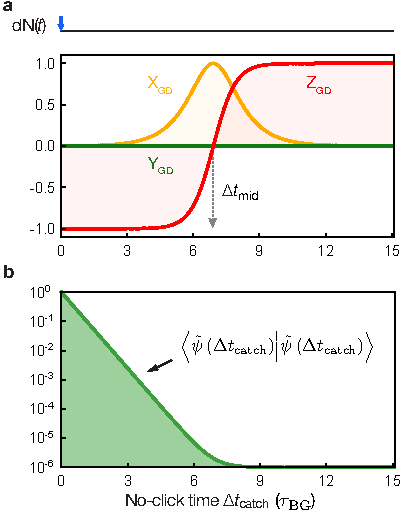
\includegraphics[scale=1.4]{qmjump/ideal_jump}
\par\end{centering}
\caption[Conditional no-click evolution of the jump from $\G$ to $\D$: ideal
photodetection theory.]{\textbf{\label{fig:Conditional-no-click-evolution}Conditional no-click
evolution of the jump from $\G$ to $\D$: ideal photodetection theory.
a, }A typical quantum trajectory for a jump from $\G$ to $\D$ represented
as the GD Bloch vector ($X_{\mathrm{GD}}$, $Y_{\mathrm{GD}}$, $Z_{\mathrm{GD}}$),
conditioned on \emph{no }clicks, $\dN\left(t\right)=0$, for duration
$\deltatcatch$. The Rabi drives are $\Omega_{\mathrm{DG}}=10^{-5}$
and $\Omega_{\mathrm{BG}}=0.1$ in units of the decay rate $\gamma_{\mathrm{B}}$.
Time axis is scaled in units of the mean time between detector clicks,
$\tau_{\mathrm{BG}}=(\Omega_{{\rm BG}}^{2}/\gamma_{\mathrm{B}})^{-1}$.
Time scale of the jump flight is the mid-flight time $\Delta t_{\mathrm{mid}}$,
defined by $Z_{\mathrm{GD}}=0$. \textbf{b,} Log plot of the norm
of the un-normalized no-click state, $\braket{\tilde{\psi}\left(\Delta t_{\mathrm{catch}}\right)}{\tilde{\psi}\left(\Delta t_{\mathrm{catch}}\right)}$,
as a function of $\deltatcatch$, in units of $\tau_{\mathrm{BG}}$.
Parameters of the plot correspond to those of panel a. }
\end{figure}


\paragraph{Remarks on the state evolution. }

The evolution of the GD manifold Bloch vector ($X_{\mathrm{GD}}\left(\deltatcatch\right),$
$Y_{\mathrm{GD}}\left(\deltatcatch\right),$ $Z_{\mathrm{GD}}\left(\deltatcatch\right)$)
conditioned on \emph{no }clicks, $\dN\left(\deltatcatch\right)=0$,
for duration $\deltatcatch$, is plotted in Fig.~\ref{fig:Conditional-no-click-evolution}a.
The partial tomogram visually shows that the predicted evolution of
the quantum jump from $\ket{\mathrm{G}}$ to $\ket{\mathrm{D}}$ is
continuous and coherent, $X_{\mathrm{GD}}^{2}+Y_{\mathrm{GD}}^{2}+Z_{\mathrm{GD}}^{2}=1$
for all no-click times, $\deltatcatch$. The measurement record, $\dN$,
and the predicted trajectory is identical for any two jumps from $\G$
to $\D$. The time axis has been scaled in units of the mean time,
$\tau_{\mathrm{BG}}=(\Omega_{{\rm BG}}^{2}/\gamma_{\mathrm{B}})^{-1}$,
between photon detector clicks. This time can also be understood as
the inverse of the information-gain rate of the measurement about
the G level. To expand on this, for definitiveness, consider the situation
where the atom is initialized in $\G$, but this information is not
shared with the observer operating the photon detector. By measurement,
how long does it take the observer to statistically deduce that the
atom is in $\G$ or not?  The measurement drive $\Omega_{\mathrm{BG}}$
is actuated and the observer  monitors the detector for clicks. If
the atom is in $\G,$ on average, the detector records a click after
time $\tau_{\mathrm{BG}}$, and informs the observer that the atom
is definitively in $\G$. Alternatively, if the atom was initialized
in $\D,$ no clicks would be recorded. As the detector does not record
a click for durations longer than $\tau_{{\rm BG}}$, the observer
becomes increasingly confident that the atom could not be in $\G$
since it becomes exponentially unlikely that a click has not yet been
observed, see Fig.~\ref{fig:Conditional-no-click-evolution}b, and
the alternative conclusion, that the atom is in $\D$, becomes increasingly
likely. Although this information-gain consideration is carried out
from the point of view of the observer, and with classical measurements
would bear no consequence for the objective state of the system, with
quantum measurements the gain of information about the system by virtue
of a measurement is necessarily accompanied by a result-correlated
state-disturbance (back-action). In Hilbert space, the disturbance
can be viewed as a \emph{measurement-backaction effective force},
as discussed in the following subsection, Sec.~\ref{subsec:Knowledge-driven-force-in}.

\paragraph{Probability of no-click record.}

Fig.~\ref{fig:Conditional-no-click-evolution}b shows a plot of the
conditional no-click state norm, $\braket{\psi\left(\deltatcatch\right)}{\psi\left(\deltatcatch\right)}$,
as a function of the no-click duration, $\deltatcatch$. The norm
initially decays exponentially with a time-constant $\tau_{{\rm BG}}$,
during which time, the atom remains essentially in $\G$, as indicated
by the $Z_{{\rm GD}}$ Bloch component in panel a, which is roughly
equal to $-1$. However, as the no-click duration approaches  mid-flight
time of the jump, $\deltatcatch\approx\Delta t_{{\rm mid}}$, the
decay of the norm slows down dramatically, since the atom transitions
from $\G$ to $\D$, in which state one can stop expecting the rapid
occurrence of clicks. The quantum jump from $\G$ to $\D$ can be
observed in the tomogram shown in panel (a). For no-click duration
$\deltatcatch\gg\Delta t_{{\rm mid}}$, the decay of the norm initially
appears flat, however, on longer time-scales (not shown) it is seen
that it also follows an exponential decay law with a much longer time
constant, $\tau_{{\rm DG}}\gg\tau_{{\rm BG}}$, corresponding to the
waiting-time for the jump back down, from $\D$ to $\G$.

\paragraph{\textit{\emph{Application of the photon counting model to the experiment.}}}

The photon-counting theory presented in this section provides the
background to the experiment along with a link to the original ion
experiments. It captures a core set of the ideas, even though the
monitoring of $|{\rm B\rangle}$ implemented in the experiment is
diffusive — the opposite limit of the point-process description presented
here, see Sec.~\ref{sec:Heterodyne-monitoring-of}. Nevertheless,
the photon-counting theory even provides a quantitative first approximation
of the experimental results. For definitiveness, consider the flight
of the quantum jump shown in Fig.~\ref{fig:catch}b. The measured
mid-flight time, $\Delta t_{\mathrm{mid}}=3.95~\mathrm{\mu s}$, is
predicted, in a first approximation, by Eq.~(\ref{eq:t_mid_coherent}).
Using the (independently measured) values of the experimental parameters,
summarized in Table~\ref{tab:system-params} (setting $\Omega_{\mathrm{BG}}$
equal to $\Omega_{\mathrm{B0}}=2\pi\times1.2$~MHz, the BG drive
when the atom is not in $\ket{\rm B}$) and extracting the effective
measurement rate of $|{\rm B\rangle}$, $\gamma_{\mathrm{B}}=2\pi\times9.0$~MHz
(which follows from Eq.~(\ref{eq:GammaBG}) where $\Gamma_{\mathrm{BG}}=2\pi\times1.01$~MHz,
the average click rate on the BG transition), Eq.~(\ref{eq:t_mid_coherent})
predicts $\Delta t_{{\rm mid}}\approx4.3~\mathrm{\mu s}$ — in fair
agreement with the observed value $\Delta t_{{\rm mid}}=3.95~\mathrm{\mu s}$.
The photodetection theory presented in in Sec.~\ref{subsec:Incoherent-Bright-drive}
further improves the agreement. These calculations serve to generally
illustrate the theory and ideas of the experiment; the quantitative
comparison between theory and experiment is only presented in Sec.~\ref{subsec:Comparison-between-theory}.

\subsection{Measurement-backaction effective force in the absence of the Dark
Rabi drive\label{subsec:Knowledge-driven-force-in}}

While in Sec.~\ref{sec:thry:3lvl-atom-simple-log} we considered
the coherent dynamics of the three-level atom in the presence of  both
unitary evolution, due to the Rabi drive $\Odg$, and the competing
non-unitary state collapse, due to the measurement, in this subsection,
we examine the simpler case where only measurement dynamics are at
play, i.e., $\Odg=0$. In this simpler situation, some important features
of the measurement, consisting of the Rabi drive $\Obg$ and the monitoring
of the B level at the rate $\gamma_{{\rm B}}$, are more easily discussed.
In particular, we pay attention to the notion of a\emph{ measurement-backaction
effective force}, the special force that unavoidably disturbs of the
quantum state due to the measurement. 

For definitiveness, consider the situation where  the three-level
atom is prepared in an initial superposition involving the G and D
levels, $\ket{\psi\left(0\right)}=\mathcal{N}\left(\G+\epsilon\D\right)$,
where $\epsilon\ll1$ and $\mathcal{N}$ is the ket normalization
factor; for simplicity, assume $\D$ is completely decoupled form
the environment, $\gamma_{{\rm D}}=0$. To measure the atom, only
the Rabi drive $\Obg$ is turned on. One of two qualitatively distinct
measurement records is observed: either clicks are recorded indefinitely
or no clicks are ever recorded, which can qualitatively be understood
in view of the following considerations. When the BG drive is first
turned on, some of the initial population from the G level is transferred
to the B level due to the steering force of $\Obg$. However, even
as a tiny amount of population is deposited in $\B$, the strong coupling
with the environment and the photodetector dampens the transfer and
quickly yields the detection of a click, with probability $\wp_{1}\left(\dt\right)=\left\langle \hat{c}_{{\rm B}}^{\dagger}\hat{c}_{{\rm B}}\right\rangle \left(t\right)\dt$,
where $\hat{c}_{\mathrm{B}}=\sqrt{\gamma_{{\rm B}}}\kb{\mathrm{G}}{\mathrm{B}}$
is the  jump operator. The click resets the atom to the ground state,
$\G$. Once the atom is completely in $\G$, the amplitude of $\D$
is zero, and since $\Odg=0$, the atom can never transition to $\D$
subsequently. The remainder of the history proceeds as described above,
the atom remains predominantly in $\G$ and continues to fluoresce
though the partial excitation and subsequent relaxation of $\B$,
by means of $\Obg$ and the detection, $\gamma_{{\rm B}}$, respectively.
In this way, the Dehmelt electron scheme implements a measurement
with result $\G$, occurring with an approximate probability $1-\epsilon^{2}$.
The alternative set of trajectories, where no clicks are observed
is quantitatively analyzed in the following, and occur with approximate
probability $\epsilon^{2}$.

\paragraph{No-click trajectory. }

The \emph{normalized} state of the three-level atom conditioned on
no-clicks, \footnote{Notationally, we employ capital letters for the coefficients of the
normalized sate, and lower-case letters for those of the un-normalized
state.} 
\begin{equation}
\ket{\psi_{I=0}\left(t\right)}=\cgn\left(t\right)\G+\cbn\left(t\right)\B+\cdn\left(t\right)\D\,,\label{eq:psiPhotonNL}
\end{equation}
evolves according to the non-linear Schrödinger equation, see Eq.~(\ref{eq:psiPhotonNoClick}),
\begin{equation}
\frac{\mathrm{d}}{\mathrm{d}t}\ket{\psi_{I=0}\left(t\right)}=\left(-i\hat{H}-\half\hat{c}_{{\rm B}}^{\dagger}\hat{c}_{{\rm B}}+\half\left\langle \hat{c}_{{\rm B}}^{\dagger}\hat{c}_{{\rm B}}\right\rangle \left(t\right)\right)\ket{\psi_{I=0}\left(t\right)}\:,\label{eq:NL-SSe-Cond-3}
\end{equation}
which in terms of the normalized state coefficients ($\cgn,\cbn$,
and $\cdn$) yields the set of coupled non-linear equations,
\begin{align}
\ddt\cbn\left(t\right)= & \frac{1}{2}\gamma_{{\rm B}}\cbn\left(t\right)^{3}+\frac{1}{2}\Omega_{{\rm BG}}\cgn\left(t\right)-\half\gamma_{{\rm B}}\cbn\left(t\right),\label{eq:Cbn}\\
\ddt\cgn\left(t\right)= & \frac{1}{2}\gamma_{{\rm B}}\cbn\left(t\right)^{2}\cgn\left(t\right)-\frac{1}{2}\Omega_{{\rm BG}}\cbn\left(t\right),\label{eq:Cgn}\\
\ddt\cdn\left(t\right)= & \frac{1}{2}\gamma_{{\rm B}}\cbn\left(t\right)^{2}\cdn\left(t\right),\label{eq:Cdn}
\end{align}
The measurement terms in Eqs.~(\ref{eq:Cbn})-(\ref{eq:Cdn}) associated
with information gain are the non-linear ones. As discussed in Sec.~\ref{sec:Quantum-trajectory-theory},
they originate from the normalization term in the conditional state
update and give rise to non-unitary state dynamics, resulting in a
drastic departure from the usual Schrödinger equation. To analyze
their effect and gain some physical intuition, we introduce a graphical
representation of the Hilbert space of the three-level atom.

\paragraph{$\mathbb{R}$-qutrit sphere representation. }

It follows from the real coefficients of Eqs.~(\ref{eq:Cbn})-(\ref{eq:Cdn})
and the initial conditions that $\cgn,\cbn,$ and $\cdn$ are constrained
to be real. Hence a pure state of the atom admits a geometrical representation
as a point on the unit sphere defined by the state norm condition
$\cbn^{2}+\cgn^{2}+\cdn^{2}=1$, see Fig.~\ref{fig:R-qutrit-sphere-representation.}.
We nickname this representation the '$\mathbb{R}$-qutrit sphere'.
Unlike the Bloch sphere representation where orthogonal state vectors
are represented by \emph{antiparallel} vectors, in the $\mathbb{R}$-qutrit
sphere representation, orthogonal state vectors are actually represented
by orthogonal vectors, extending from the origin to the surface of
the sphere. Notably, the sphere contains states of the two-level sub-manifolds
that are \emph{not} represented on the Bloch sphere, those with a
``global phase.''\footnote{The special unitary Lie group $SU(2)$ is not isomorphic to the special
orthogonal Lie group $SO(3)$, but is a double cover of it.} The addition of the third level allows, in general, the observation
of the global phase because it can be measured relative to the phase
of the third level. Consequently, a Rabi rotation between two levels
is no longer $2\pi$ periodic but $4\pi$ periodic.  Unitary evolution
is represented by rotations on the sphere; for instance, the evolution
due to the Bright Rabi drive, $\Obg$, is a rotation about the D axis,
and the corresponding infinitesimal-state-change vector field, $\mathrm{d}\ket{\psi}\left(\Obg\right)=\frac{1}{2}\left(\cgn\B-\cbn\G\right)\Obg\dt$,
is plotted on the surface of the sphere in Fig.~\ref{fig:R-qutrit-sphere-representation.}.
Note that the length of the vectors is largest at the GB equator and
approaches zero toward the D poles. The vector field representation
is useful in the analysis of the non-linear measurement-backaction
effective force  due to the renormalization terms and we hope can
provide a more intuitive understanding of the interplay between the
coherent Rabi and the stochastic measurement dynamics.  Before elaborating
on the geometrical representation of the measurement dynamics, it
is useful to first algebraically solve Eqs.~(\ref{eq:Cbn})-(\ref{eq:Cdn}).

\begin{figure}
\begin{centering}
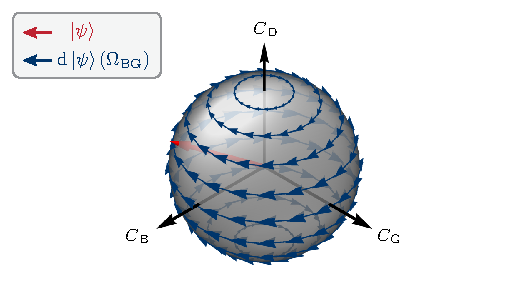
\includegraphics[scale=1.5]{qmjump/knowledge_sphere}
\par\end{centering}
\caption[Geometrical representation of a qutrit state with real coefficients:\textbf{
$\mathbb{\mathbb{R}}$}-qutrit sphere]{\label{fig:R-qutrit-sphere-representation.}\textbf{Geometrical representation
of a qutrit state with real coefficients:} $\mathbb{\mathbb{R}}$\textbf{-qutrit
sphere. }Geometric representation of the Hilbert space of pure states
of a qutrit, $\ket{\psi}=\cbn\B+\cgn\G+\cdn\D$, with real-valued
coefficients, notably isomorphic to the special orthogonal group $SO\left(3\right)$.
Overlaid vector field represents the infinitesimal state change, $\mathrm{d}\ket{\psi}$,
due to the Rabi drive $\Omega_{{\rm BG}}.$}
\end{figure}


\paragraph{Measurement-backaction  force steers atom towards $\D$. }

Although there is no Rabi drive or measurement directly applied to
the Dark level, conditioned on not detecting a click, according to
Eq.~(\ref{eq:Cdn}), a force is nonetheless exerted by the B-level
monitoring that steers the atom toward the Dark level. Specifically,
the rate of change of the D level amplitude, $\ddt\cdn$, is given
by an anti-damping term with a state-dependent rate proportional to
the B level population, $\cbn\left(t\right)^{2}$, and measurement
rate, $\gamma_{{\rm B}}$. Solving Eq.~(\ref{eq:Cdn}), one finds
\begin{equation}
\cdn\left(t\right)=\cdn\left(0\right)\exp\left(\int_{0}^{t}\mathrm{d}t'\frac{1}{2}\gamma_{{\rm B}}\cbn\left(t\right)^{2}\right)\,.\label{eq:Cdsol}
\end{equation}
In this sense, the renormalization of the conditional state amounts
to a (non-unitary) measurement-backaction force on $\D$, which is
linked to the population of $\B.$ To explicitly solve Eq.~(\ref{eq:Cdsol}),
we need to solve the remaining equations, Eqs.~(\ref{eq:Cbn}) and
(\ref{eq:Cgn}). 

\paragraph{Adiabatic elimination of the Bright state dynamics.}

Because Eq.~(\ref{eq:Cbn}) is non-linear, we consider the B level
dynamics and their adiabatic elimination with greater care. Eq.~(\ref{eq:Cbn}),
contains both a damping, $-\half\gamma_{{\rm B}}\cbn$, and an anti-damping,
$\frac{1}{2}\gamma_{{\rm B}}\cbn{}^{3}$, term. These cancel out perfectly
only if the atom is either entirely in $\B$, $\cbn=\pm1$, or not
at all in $\B$, $\cbn=0$; otherwise, $\left|\cbn\right|<1$, the
damping dominates, steering $\cbn$ in the direction of zero. In the
extreme case, where $\Omega_{{\rm BG}}=0$, one can explicitly solve
the B level dynamics, $\cbn\left(t\right)^{2}=\left[1+\left(\cbn\left(0\right)^{-2}-1\right)\exp\left(\gamma_{{\rm B}}t\right)\right]^{-1},$
which for small initial populations, $\cbn\left(0\right)^{2}\ll1$
rapidly decays to a stable zero equilibrium at a rate $\frac{1}{2}\gamma_{{\rm B}}$,
$\cbn\left(t\right)\approx\cbn\left(0\right)\exp\left(-\frac{1}{2}\gamma_{{\rm B}}t\right)$.
Since $\gamma_{{\rm B}}$ is the fastest timescale in the problem
and the B dynamics are convergent, we can adiabatically eliminate
$\cbn$ by setting $\ddt\cbn\left(t\right)=0$; solving the cubic
equation, one finds three solution branches,
\begin{equation}
\cbnb\left(t\right)=\begin{cases}
-1-\frac{\Obg}{2\gamma_{{\rm B}}}\cgn\left(t\right)+\mathcal{O}\left(\left(\Obg/\gamma_{{\rm B}}\right)^{2}\right)\\
1-\frac{\Obg}{2\gamma_{{\rm B}}}\cgn\left(t\right)+\mathcal{O}\left(\left(\Obg/\gamma_{{\rm B}}\right)^{2}\right)\\
\frac{\Obg}{\gamma_{{\rm B}}}\cgn\left(t\right)+\mathcal{O}\left(\left(\Obg/\gamma_{{\rm B}}\right)^{3}\right)\,.
\end{cases}\label{eq:Cb-bar}
\end{equation}
Operating the three-level atom in the limit where the $\B$ level
is never appreciably populated, we employ the third solution branch,
$\cbnb\left(t\right)=\frac{\Obg}{\gamma_{{\rm B}}}\cgn\left(t\right)$,
in Eq.~(\ref{eq:Cgn}) to find the effective equation of motion for
the G level dynamics, 
\begin{equation}
\ddt\cgn\left(t\right)=-\tau_{\mathrm{BG}}^{-1}\left[1-\cgn\left(t\right)^{2}\right]\cgn\left(t\right),\label{eq:ddtCGn}
\end{equation}
which are now completely decoupled from the other levels. In Eq.~(\ref{eq:ddtCGn}),
we identify a damping and an anti-damping term with a constant and
G-population dependent, $\cgn^{2}$, rate, respectively. The scale
of both terms is given by the parameter $\tau_{\mathrm{BG}}^{-1}=\Omega_{{\rm BG}}^{2}/2\gamma_{\mathrm{B}}$,
which is the expected rate of clicks when the atom is in $\G$. By
eliminating the B level, we have obtained an explicit relation for
the effective monitoring of the G level, which occurs at a rate $\tau_{{\rm BG}}^{-1}$,
which can also be interpreted as the quantum Zeno rate \citep{Misra1977,Gambetta2008-qm-traj,Matsuzaki2010,Vijay2011,Slichter2016-T1vsNbar,Harrington2017,Hacohen-Gourgy2018}.
The numerator $\Obg^{2}$ is proportional to the population transfer
rate from $\G$ to $\B$ while the denominator $\gamma_{{\rm B}}$
gives the rate of projection from $\B$ to $\G$. Solving Eq.~(\ref{eq:ddtCGn})
and substituting its solution in Eq.~(\ref{eq:Cdsol}), one finds
\begin{figure}
\begin{centering}
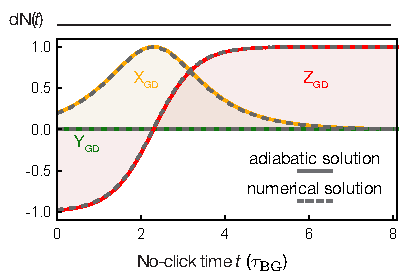
\includegraphics[scale=1.5]{qmjump/knowledge_img1}
\par\end{centering}
\caption[Adiabatic solution for the no-click GD manifold trajectory of a superposition
state measured with $\Odg=0$]{\textbf{\label{fig:3:adiabatic-sol}Adiabatic solution for the no-click
GD manifold trajectory of a superposition state measured with }$\Odg=0$\textbf{.
}Adiabatic-approximation (solid lines) and numerical (dashed lines)
solution for the partial tomogram of the GD manifold of the no-click
quantum trajectory of an initial superposition state $\ket{\psi\left(0\right)}=\mathcal{N}\left(\G+\epsilon\D\right)$,
where $\epsilon=0.1$ and $\mathcal{N}=\left(1+\epsilon^{2}\right)^{-1/2}$.
The Bright Rabi drive is $\Obg=0.1$, in units of the decay rate $\gamma_{{\rm B}}$.
Time axis scaled in units of $\tau_{\mathrm{BG}}=\left(\Obg^{2}/\gamma_{{\rm BG}}\right)^{-1}.$}
\end{figure}
\begin{align}
\cgn\left(t\right)^{2}= & \frac{p_{{\rm G}}}{p_{{\rm G}}+\left(1-p_{{\rm G}}\right)e^{2t/\tau_{{\rm BG}}}}\,,\label{eq:Cgnoclicksol}\\
\cdn\left(t\right)^{2}= & \frac{p_{{\rm D}}e^{t/\tau_{{\rm BG}}}}{p_{{\rm D}}+\left(1-p_{{\rm D}}\right)e^{2t/\tau_{{\rm BG}}}}\,,\label{eq:CdNoClickSol}
\end{align}
where $p_{{\rm G}}\equiv\cgn\left(0\right)^{2}$ and $p_{{\rm D}}\equiv\cdn\left(0\right)^{2}$
are the initial conditions. Note, for $p_{{\rm D}}=0$, the above
solution for $\cdn$ is always zero. The evolution of the GD Bloch
vector conditioned on no clicks for the initial state $\ket{\psi\left(0\right)}=\mathcal{N}\left(\G+\epsilon\D\right)$
is obtained by substituting Eq.~(\ref{eq:Cgnoclicksol}) and (\ref{eq:CdNoClickSol})
in Eqs.~(\ref{eqn:Z})-(\ref{eqn:Y}), 
\begin{align}
{\rm Z}_{{\rm GD}}(t) & ={\rm tanh}\left[t/\tau_{{\rm BG}}+\mathrm{arctanh}\left[{\rm Z}_{{\rm GD}}(0)\right]\right],\label{eq:Zgd-Adi}\\
{\rm X}_{{\rm GD}}(t) & ={\rm sech}\left[t/\tau_{{\rm BG}}+\mathrm{arctanh}\left[{\rm Z}_{{\rm GD}}(0)\right]\right],\\
{\rm Y}_{{\rm GD}}(t) & =0.\label{eq:Ygd-Adi}
\end{align}
We note that a few results of this subsection, especially Eqs.~(\ref{eq:Zgd-Adi})-(\ref{eq:Ygd-Adi}),
bear resemblance to results from Sec.~\ref{sec:thry:3lvl-atom-simple-log},
yet we stress that  the two situations are fundamentally distinct,
and the resemblance must be considered with care. For instance, we
note that the mid-flight time $\Delta t_{\mathrm{mid}}$ cannot be
recovered from the simpler situation considered here, where no quantum
jumps occur and there is no competition between unitary dynamics due
to $\Omega_{{\rm DG}}$ and the measurement. 

In Fig.~\ref{fig:3:adiabatic-sol}a, we plot the adiabatic-approximation
solution to the non-linear Schrödinger evolution, Eq.~(\ref{eq:NL-SSe-Cond-3}),
for the GD manifold Bloch vector conditioned on no clicks, Eqs.~(\ref{eq:Zgd-Adi})-(\ref{eq:Ygd-Adi}),
obtained in the limit $\Obg\ll\gamma_{B}$. Overlaid (dashed lines)
is the corresponding numerically calculated solution to Eq.~(\ref{eq:NL-SSe-Cond-3}).
Even for modest separation of timescales, $\Obg/\gamma_{{\rm B}}=0.1$
in the plot, the two solutions appear nearly indistinguishable. The
initial atom state, $\epsilon=0.1$, is gradually projected to $\D$
on a timescale given by $\tau_{{\rm BG}}$ and evolves in a characteristically
non-unitary manner. Notably, the state remains pure at all times,
and in the limit $t\gg\tau_{{\rm BG}}$ remains essentially in $\D$,
indefinitely. Importantly, for times $t$ on the other of $\tau_{{\rm BG}}$,
the projection can (but need not) be interrupted by the detection
of a click, which would project the state to $\G$, and occurs with
total probability $\approx1-\epsilon^{2}$. 
\begin{figure}
\begin{centering}
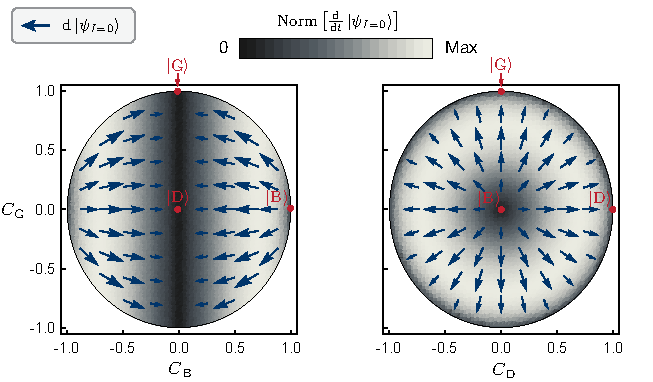
\includegraphics[scale=1.4]{qmjump/knowledge_img2}
\par\end{centering}
\caption[Geometrical representation of the no-click measurement-backaction
force for $\Obg=0$]{\textbf{\label{fig:Knowledge-driven-force-in-1}Geometrical representation
of the no-click measurement-backaction  force for $\Obg=0$.} Shown
are two projections of $\mathbb{\mathbb{\mathbb{R}}}$-qutrit sphere
overlaid with the measurement-force vector field, $\frac{\mathrm{d}}{\mathrm{d}t}\ket{\psi_{I=0}}$,
due to the monitoring of the B level with $\Obg=0$. Color of density
plot indicates the relative magnitude of the change, $\mathrm{Norm}\left[\frac{\mathrm{d}}{\mathrm{d}t}\ket{\psi_{I=0}}\right]$.}
\end{figure}


\paragraph{Hilbert space representation of the measurement dynamics.}

It is useful to consider a geometric representation of the measurement
dynamics and in particular of the non-linear measurement-backaction
force. For simplicity, first consider the measurement force due only
to the monitoring of the B level, in the absence of the Bright Rabi
drive, $\Obg=0$. This  force can be represented as a vector field
on the surface of the $\mathbb{R}$-qutrit sphere, see Fig.~\ref{fig:Knowledge-driven-force-in-1}.
The vector field is calculated from Eqs.~(\ref{eq:Zgd-Adi})-(\ref{eq:Ygd-Adi})
for the change in the state conditioned on detecting no clicks, 
\begin{equation}
\frac{\mathrm{d}}{\mathrm{d}t}\ket{\psi_{I=0}}=\frac{1}{2}\gamma_{{\rm B}}\cbn{}^{2}\begin{pmatrix}\cbn-1\\
\cgn\\
\cdn
\end{pmatrix}\,.\label{eq:ddtPsiI-vec}
\end{equation}
The colormap in Fig.~\ref{fig:Knowledge-driven-force-in-1} depicts
the relative magnitude of the change, $\mathrm{Norm}\left[\frac{\mathrm{d}}{\mathrm{d}t}\ket{\psi_{I=0}}\right],$
which we note is only zero in two special cases: i) when the atom
is $\pm\B$, corresponding to the points $\left(\pm1,0,0\right),$
and ii) when the atom is in a\emph{ }state involving exclusively $\G$
and $\D$ but not $\B$. The latter is special in that it corresponds
to an entire manifold of states, the GD equatorial circle, which can
be visually recognized in Fig.~\ref{fig:Knowledge-driven-force-in-1}
as the dark vertical stripe at the center of the left panel and the
dark circular perimeter of the disk in the right panel. All other
states, not covered under the latter two cases, are superpositions
involving $\B$. From the vector field plot, it is evident that these
states are guided by the force away from the $\B$ poles and toward
the GD equator. It is precisely this feature of the measurement force
that results in the gradual projection of the state conditioned on
no clicks — it is the unavoidable disturbance of the atom due to the
information-gain of the no-click measurement outcomes, which lead
the observer to gradually learn that the atom is not in $\D$, thus
resulting in the increased likelihood that it is in $\G$ or $\D$.
This dynamics embody the message of the Chapter~\ref{chap:Quantum-Trajectory-Theory}
epigraph, ``In quantum physics you don't see what you get, you get
what you see.''

\begin{figure}
\begin{centering}
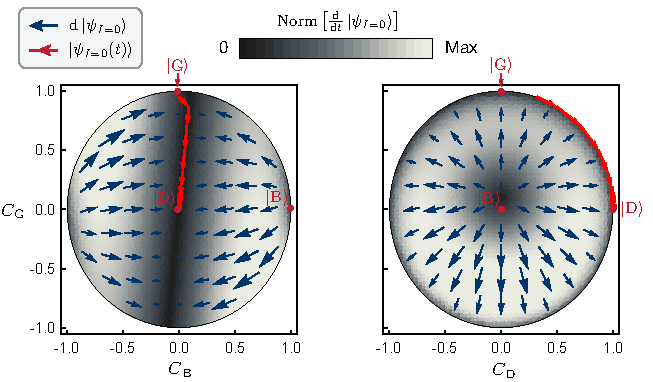
\includegraphics[scale=1.4]{qmjump/knowledge_img3}
\par\end{centering}
\caption[Geometrical representation of the measurement-backaction force and
a no-click trajectory with $\Obg=0.1\gamma_{{\rm B}}$]{\textbf{\label{fig:Knowledge-driven-force-in-2}Geometrical representation
of the measurement-backaction force and a no-click trajectory with
$\Obg=0.1\gamma_{{\rm B}}$.}  Two projections of the $\mathbb{\mathbb{\mathbb{R}}}$-qutrit
sphere overlaid with the measurement-force vector field $\frac{\mathrm{d}}{\mathrm{d}t}\ket{\psi_{I=0}}$
(blue arrows) and the path of the quantum trajectory from Fig.~(\ref{fig:3:adiabatic-sol})
(red arrows), depicting the gradual projection of a superposition
state to $\D$ conditioned on no clicks. Density plot indicates relative
field magnitude, $\mathrm{Norm}\left[\frac{\mathrm{d}}{\mathrm{d}t}\ket{\psi_{I=0}}\right]$.}
\end{figure}

In Fig.~\ref{fig:Knowledge-driven-force-in-2}, we plot the measurement
vector field in the presence of the Bright Rabi drive $\Omega_{\mathrm{BG}}$,
\begin{equation}
\frac{\mathrm{d}}{\mathrm{d}t}\ket{\psi_{I=0}}=\frac{1}{2}\gamma_{{\rm B}}\cbn{}^{2}\begin{pmatrix}\cbn-1\\
\cgn\\
\cdn
\end{pmatrix}+\frac{1}{2}\Obg\begin{pmatrix}\cgn\\
-\cbn\\
0
\end{pmatrix}\,,\label{eq:ddtPsiI-vec-1}
\end{equation}
with $\Obg=0.1\gamma_{{\rm B}}$. The Bright Rabi drive, visually
represented on the $\mathbb{R}$-qutrit sphere in Fig.~\ref{fig:R-qutrit-sphere-representation.},
perturbs the measurement field, shown in Fig.~\ref{fig:Knowledge-driven-force-in-1},
by linking the B and G levels and lifting the degeneracy of the measurement,
represented in GD equator. Visually, this is evident in the tilt of
the vertical dark stripe in the center of the left-panel colormap.
In the right panel, it is also evident that $\B$ is no longer an
equilibrium point; the equilibrium has been shifted in the direction
of $\G$ by an amount proportional $\Obg/\gamma_{{\rm B}},$ see Eq.~(\ref{eq:Cb-bar}),
and made metastable. The red arrows depict the path of the quantum
trajectory in Hilbert of the gradual projection of an initial superposition
state of $\G$ and $\D$, for the same parameters as employed in Fig.~(\ref{fig:3:adiabatic-sol}),
where $\epsilon=0.1$. Initially, the state is quickly steered in
the direction of $\B$ by the force of $\Obg$. However, as the state
moves in the direction of $\B$, the motion is quickly opposed by
the no-click measurement-backaction force, which grows larger in amplitude
in this direction. The two forces do not precisely cancel each other
out, because of the slight mismatch in angles. The net force, albeit
small, steers the atom towards the GD equator and with a slight tilt
toward $\D$. The opposition of the $\Obg$ drive and the measurement
back-action ``trap'' the state in the ridge where the two forces
nearly cancel each other out, the nearly vertical dark stripe in the
left panel, and the small angular mismatch slowly carries the state
in the direction of $\D$, an equilibirum point, where all forces
are zero.


\subsection{Incoherent Bright drive and Dark drive off\label{subsec:Incoherent-Bright-drive}}

In this section, we consider the case of quantum jumps in the three-level
atom subject to photodetection and an incoherent Bright drive, rather
than a Rabi one, see Sec.~\ref{sec:thry:3lvl-atom-simple-log}. The
situation analyzed in this section is somewhat more analogous to the
cQED experiment where the Bright Rabi drive consists of a bi-chromatic
tone that unconditionally addresses the BG transition, independent
of the population of the readout cavity, necessitated by the  dispersive
pull of the readout cavity on the BG frequency. The bi-chromatic drive
effectively acts as an incoherent drive. The incoherent Bright drive
photodetection theory presented here sheds some further light on the
dynamics of the quantum jump from $\G$ to $\D$. Features such as
the non-zero coherence, $X_{{\rm GD}}$, and in the limit $\deltatcatch\gg\Delta t_{{\rm mid}}$
are discussed.\footnote{The following derivation is due to H.J. Carmichael and R. Gutierrez-Jauregui.}

Replacing the coherent Rabi drive $\Omega_{{\rm BG}}$ by an incoherent
drive $\Gamma_{{\rm BG}}$ in  the master equation of the three-level
atom in the interaction picture, Eq.~(\ref{eq:PhotonLindblad}) becomes
\begin{equation}
\frac{\mathrm{d}\rho}{\mathrm{d}t}=(i\hbar)^{-1}[\hat{H}_{{\rm drive}},\rho]+\Gamma_{{\rm BG}}{\cal D}\left[\kb{\rm B}{\rm G}\right]\rho+(\gamma_{{\rm B}}+\Gamma_{{\rm BG}}){\cal D}\left[\kb{\rm G}{\rm B}\right]\rho+\gamma_{{\rm D}}{\cal D}\left[\kb{\rm G}{\rm D}\right]\rho,
\end{equation}
and Eq.~(\ref{eq:ClickHeff}) becomes
\begin{equation}
\hat{H}_{{\rm drive}}=i\hbar\frac{\Omega_{{\rm DG}}}{2}\big(\kb{\rm D}{\rm G}-\kb{\rm G}{\rm D}\big).
\end{equation}
The strong-monitoring assumption, $\tau_{{\rm BG}}^{-1}\ll\gamma_{{\rm B}}$,
is also carried over from Sec.~\ref{sec:thry:3lvl-atom-simple-log}
by assuming $\Gamma_{{\rm BG}}\ll\gamma_{{\rm B}}$, i.e., the time
between clicks in fluorescence is essentially the same as the time
separating photon absorptions from the incoherent drive, as absorption
is rapidly followed by fluorescence ($\gamma_{{\rm B}}+\Gamma_{{\rm BG}}\gg\Gamma_{{\rm BG}}$).
This brings a useful simplification, since, following each reset to
$\G$, the unnormalized state evolves in the GD-subspace, 
\begin{equation}
i\hbar\frac{\mathrm{d}\ket{\tilde{\psi}}}{\mathrm{d}\Delta t_{{\rm catch}}}=\left(\hat{H}_{{\rm drive}}-i\hbar\frac{\Gamma_{{\rm BG}}}{2}\kb{\rm G}{\rm G}-i\hbar\frac{\gamma_{{\rm D}}}{2}\kb{\rm D}{\rm D}\right)\ket{\tilde{\psi}},
\end{equation}
thus replacing Eqs.~(\ref{eqn:3x3_system}) and (\ref{eqn:W_DG_equation_coherent})
by the simpler $2\times2$ system 
\begin{equation}
\frac{\mathrm{d}}{\mathrm{d}\Delta t_{{\rm catch}}}\begin{pmatrix}\cg\\
\cd
\end{pmatrix}=\frac{1}{2}\left(\begin{matrix}-\Gamma_{{\rm BG}} & -\Omega_{{\rm DG}}\\
\Omega_{{\rm DG}} & -\gamma_{{\rm D}}
\end{matrix}\right)\begin{pmatrix}\cg\\
\cd
\end{pmatrix},
\end{equation}
and, in the limit $\gamma_{{\rm D}}\ll\Gamma_{{\rm BG}}$, the equation
of motion for $W_{{\rm DG}}$, defined in Eq.~(\ref{eqn:W_DG_definition}),
is
\begin{equation}
\frac{\mathrm{d}W_{{\rm DG}}}{\mathrm{d}\Delta t_{{\rm catch}}}=\frac{\Gamma_{{\rm BG}}}{2}W_{{\rm DG}}+\frac{\Omega_{{\rm DG}}}{2}(1+W_{{\rm DG}}^{2}),\label{eqn:W_DG_equation_incoherent}
\end{equation}
with solution, for $W_{{\rm DG}}(0)=0$, 
\begin{equation}
W_{{\rm DG}}(\Delta t_{{\rm catch}})=\frac{\exp\left[(V-V^{-1})\Omega_{{\rm DG}}\Delta t_{{\rm catch}}/2\right]-1}{V-V^{-1}\exp\left[(V-V^{-1})\Omega_{{\rm DG}}\Delta t_{{\rm catch}}/2\right]},\label{eqn:W_DG_incoherent}
\end{equation}
where 
\begin{equation}
V=\frac{1}{2}\frac{\Gamma_{{\rm BG}}}{\Omega_{{\rm DG}}}+\sqrt{\frac{1}{4}\left(\frac{\Gamma_{{\rm BG}}}{\Omega_{{\rm DG}}}\right)^{2}-1}.
\end{equation}
In Ref.~\citet{Ruskov2007}, a general form of the Bloch vector equations
for arbitrary amplitude of the Rabi drive was found. Inversion of
the condition $W_{{\rm DG}}(\Delta t_{{\rm mid}})=1$ gives the characteristic
time scale 
\begin{equation}
\Delta t_{{\rm mid}}=2\left[(V-V^{-1})\Omega_{{\rm DG}}\right]^{-1}\ln\left(\frac{V+1}{V^{-1}+1}\right).\label{eqn:t_mid_incoherent}
\end{equation}
Although Eqs.~(\ref{eqn:W_DG_incoherent}) and (\ref{eqn:t_mid_incoherent})
replace Eqs.~(\ref{eq:WDG-coh}) and (\ref{eq:t_mid_coherent}),
under strong monitoring, $\Gamma_{{\rm BG}}\gg\Omega_{{\rm DG}}$,
they revert to the latter with the substitution $\Omega_{{\rm BG}}^{2}/2\gamma_{{\rm B}}\to\Gamma_{{\rm BG}}/2$,;
in this way, Eqs.~(\ref{eqn:Z})–(\ref{eqn:Y}) are recovered with
the same substitution. More generally, $W_{{\rm DG}}(\Delta t_{{\rm catch}})$
goes to infinity at finite $\Delta t_{{\rm catch}}$, changes sign,
and returns from infinity to settle on the steady value $W_{{\rm DG}}(\infty)=-V$.
The singular behavior marks a trajectory passing through the north
pole of Bloch sphere. It yields the long-time solution 
\begin{equation}
{\rm Z}_{{\rm GD}}(\infty)=\sqrt{1-4\left(\frac{\Omega_{{\rm DG}}}{\Gamma_{{\rm BG}}}\right)^{2}},\qquad{\rm X}_{{\rm GD}}(\infty)=-2\frac{\Omega_{{\rm DG}}}{\Gamma_{{\rm BG}}},\qquad{\rm Y}_{{\rm GD}}(\infty)=0,\label{eq:ZGDXGD-long-term}
\end{equation}
in contrast to the perfect jump of Eqs.~(\ref{eqn:Z_approx})–(\ref{eqn:Y_approx}).
The long-term coherence and lower-than-one value of Z were observed
in the experiments, see Fig.~\ref{fig:catch}b. They can be understood
as the equilibrium point of the coherent Rabi drive $\Omega_{{\rm DG}}$
attempting to rotate the state from $\D$ back to $\G$ perfectly
balanced against the measurement-backaction force of the no-click
measurement steering the atom toward $\D$, recall discussion of the
measurement vector field, see Figs.~\ref{fig:Knowledge-driven-force-in-1}
and~\ref{fig:Knowledge-driven-force-in-2}. 

\paragraph{\textit{\emph{Dark drive off.}}}

Turing the Dark drive off shortly after a click demonstrates the connection
between the flight of a quantum jump and a projective measurement.
From the point of view of the trajectory equations, the only change
is the setting of $\Omega_{{\rm DG}}$ to zero at time $\Delta t_{{\rm on}}$
on the right-hand side of Eqs.~(\ref{eqn:W_DG_equation_coherent})
and (\ref{eqn:W_DG_equation_incoherent}). Subsequently, $W_{{\rm DG}}(\Delta t_{{\rm catch}})$
continues its exponential growth at rate $\Omega_{{\rm BG}}^{2}/2\gamma_{B}$
{[}Eq.~(\ref{eqn:W_DG_equation_coherent}){]} or $\Gamma_{{\rm BG}}/2$
{[}Eq.~(\ref{eqn:W_DG_equation_incoherent}){]}. Equations (\ref{eqn:Z})–(\ref{eqn:Y})
for the GD Bloch components still hold, but now with 
\begin{equation}
\Delta t_{{\rm mid}}=\left(\frac{\Omega_{{\rm BG}}^{2}}{2\gamma_{B}},\frac{\Gamma_{{\rm BG}}}{2}\right)^{-1}\ln\big[W_{{\rm DG}}^{-2}(\Delta t_{{\rm on}})\big].
\end{equation}
which can provide an estimate of $\Delta t'_{\mathrm{mid}}$, specifying
the time at which $Z_{\mathrm{GD}}=0$.

The evolution during $\Delta t_{\mathrm{off}}$, in the absence of
$\Omega_{\mathrm{DG}}$, in effect realizes a projective measurement
of whether the state of the atom is $\G$ or $|{\rm D}\rangle$, similar
to the one analyzed in Sec.~\ref{subsec:Knowledge-driven-force-in},
where the normalized state at $\Delta t_{{\rm on}}$ is 
\begin{equation}
\frac{|\psi(\Delta t_{{\rm on}})\rangle}{\sqrt{\mathcal{N}(\Delta t_{{\rm on}})}}=\frac{\cg(\Delta t_{{\rm on}})\G+\cd(\Delta t_{{\rm on}})\D}{\sqrt{\mathcal{N}(\Delta t_{{\rm on}})}},\label{eqn:initial_state}
\end{equation}
with $\mathcal{N}(\Delta t_{{\rm on}})=\cg^{2}(\Delta t_{{\rm on}})+\cd^{2}(\Delta t_{{\rm on}})$
the probability for the jump to reach $\Delta t_{{\rm catch}}=\Delta t_{{\rm on}}$
after a click reset to $\G$ at $\Delta t_{{\rm catch}}=0$. The probability
for the jump to continue to $\Delta t_{{\rm catch}}>\Delta t_{{\rm on}}$
(given $\Delta t_{{\rm on}}$ is reached) is then 
\begin{equation}
\frac{\mathcal{N}(\Delta t_{{\rm catch}})}{\mathcal{N}(\Delta t_{{\rm on}})}=\frac{C_{{\rm D}}^{2}(\Delta t_{{\rm on}})}{\mathcal{N}(\Delta t_{{\rm on}})}+\frac{C_{{\rm G}}^{2}(\Delta t_{{\rm on}})}{\mathcal{N}(\Delta t_{{\rm on}})}\exp\left[-\left(\frac{\Omega_{{\rm BG}}^{2}}{\gamma_{{\rm B}}},\Gamma_{{\rm BG}}\right)\Delta t_{{\rm catch}}\right].\label{eq:completion-prob}
\end{equation}


\paragraph{Completed and aborted evolutions of the jump transition.}

In this simple model, the probability for the trajectory to complete
— for the measurement to yield the result $|{\rm D}\rangle$ — is
obtained in the limit $\Delta t_{\mathrm{catch}}\rightarrow\infty$,
and, as expected, is equal to the probability to occupy the state
$|{\rm D}\rangle$ at time $\Delta t_{{\rm on}}$; i.e., the completion
probability is $P_{\mathrm{D}}(\Delta t_{{\rm on}})=C_{{\rm D}}^{2}(\Delta t_{{\rm on}})/{{\rm Norm}(\Delta t_{{\rm on}})}$.
It is helpful to illustrate this idea with an example. Consider the
catch experiment of Fig.~\ref{fig:catch}b in the absence of the
Dark Rabi drive, $\Omega_{\mathrm{DG}}$. From $Z_{\mathrm{GD}}$,
we can estimate that out of all the trajectories that pass though
the $\Delta t_{{\rm on}}$ mark approximately $P_{\mathrm{D}}(\Delta t_{{\rm on}})=(1+Z_{\mathrm{GD}}(\Delta t_{{\rm on}}))/2\approx8\%$
fully complete without an interruption. On the other hand, for those
that pass the $\Delta t'_{\mathrm{mid}}$ mark, approximately 50\%
complete. It follows from Eq.~(\ref{eq:completion-prob}), that the
probability of the evolution to complete increases the further along
the trajectory is. Although some of the jump evolutions abort at random,
importantly, every single jump evolution that completes, and is thus
recorded as a jump, follows \textit{not} a random but an identical
path in Hilbert space, i.e., a deterministic one. This path (of \textit{any}
jump) is determined by Eq.~(\ref{eqn:W_DG_incoherent}), or, in the
simpler model, by the Eqs.~(\ref{eqn:Z_approx})-(\ref{eqn:Y_approx})
for the components of the GD Bloch vector.

\section{Heterodyne monitoring of readout cavity coupled to three-level atom\label{sec:Heterodyne-monitoring-of}}

\subsection{Description of cQED experiment \label{subsec:Description-of-cQED}}

In Chapter 1, we described the cQED experiment  involving a superconducting
atom with the necessary V-shape level structure (see Fig.~\ref{fig:setup}a
or Sec.~\ref{sec:circuit-design}) subject to heterodyne monitoring
of $\B$ by means a dispersively coupled readout cavity. The three-level
atom is formed form two heavily hybridized transmon modes, which are
coupled by means of a cross-Kerr interaction to the readout cavity
in an asymmetric way, $\chi_{\mathrm{BC}}\gg\chi_{\mathrm{DC}}$.
In the following, we present the quantum trajectory description of
the heterodyne monitoring, including imperfections.

\paragraph{System Hamiltonian. }

In the lab frame, the Hamiltonian of the system is, see also Sec.~\ref{sec:circuit-design},
\begin{equation}
\hat{H}_{{\rm lab}}=\hat{H}_{0}+\hat{H}_{I}+\hat{H}_{d}\left(t\right)\,,
\end{equation}
where the Hamiltonian of the uncoupled three-level atom and cavity,
is 
\begin{equation}
\hat{H}_{0}=\hbar\omega_{{\rm DG}}\kb{\rm D}{\rm D}+\hbar\omega_{{\rm BG}}\kb{\rm B}{\rm B}+\hbar\omega_{C}\hat{c}^{\dagger}\hat{c}\,,
\end{equation}
where $\omega_{{\rm DG}}$, $\omega_{{\rm BG}}$, $\omega_{{\rm C}}$
are the Dark, Bright, and cavity mode frequency, respectively, $\hat{c}$
is the cavity amplitude operator, the atom-cavity interaction Hamiltonian
is 
\begin{equation}
\hat{H}_{I}=\hat{c}^{\dagger}\hat{c}\left[\hbar\chi_{{\rm B}}\kb{\rm B}{\rm B}+\hbar\chi_{{\rm D}}\kb{\rm D}{\rm D}\right]\:,
\end{equation}
where the shift of the cavity frequency conditioned on $\B$ ($\D$)
is $\chi_{{\rm B}}$ ($\chi_{{\rm D}}$), and the Hamiltonian of the
atom Rabi drives and readout probe tone is
\begin{align}
\hat{H}_{d}\left(t\right)= & -\frac{i\hbar}{2}\left[\kappa\sqrt{\bar{n}}\hat{c}e^{i\left(\omega_{{\rm C}}+\Delta_{{\rm R}}\right)t}+\Omega_{{\rm DG}}^{*}e^{i\left(\omega_{{\rm DG}}+\Delta_{{\rm DG}}\right)t}\kb{\rm G}{\rm D}\right.\nonumber \\
 & \left.+\Omega_{{\rm B0}}^{*}e^{i\omega_{{\rm BG}}t}\kb{\rm G}{\rm B}+\Omega_{{\rm B1}}^{*}e^{i\left(\omega_{{\rm BG}}+\Delta_{{\rm B1}}\right)t}\kb{\rm G}{\rm B}+\mathrm{H.c.}\right]\,,
\end{align}
where $\bar{n}$ is the steady state number of photons in the cavity
when driven resonantly, $\Delta_{{\rm R}}$, $\Delta_{{\rm DG}},$
and $\Delta_{{\rm B1}}$ are the drive detunings from the bare mode
frequencies. The first Bright Rabi tone, $\Omega_{{\rm B0}}$, addresses
the Bright transition when the cavity is unpopulated, while the second
tone, $\Omega_{{\rm B0}}$, addresses the BG transition  when the
cavity is populated, see frequency spectrum in Fig.~\ref{fig:setup}c.
Moving to the rotating frame at the drive frequencies, defined by
the ket transformation $\ket{\psi(t)}=U(t)\ket{\psi_{\mathrm{lab}}(t)}$,
where $U(t)=\exp\left(u\left(t\right)/i\hbar\right)$ and $u(t)=\hbar t\left[\left(\omega_{{\rm C}}+\Delta_{{\rm R}}\right)a^{\dagger}a+\omega_{{\rm BG}}\ket{\rm B}\bra{\rm B}+\left(\omega_{{\rm DG}}+\Delta_{{\rm DG}}\right)\ket{\rm D}\bra{\rm D}\right]$,
the Hamiltonian in the rotating frame is
\begin{equation}
\hat{H}\left(t\right)=\hat{H}_{{\rm R}}+\hat{H}_{{\rm drive}}\left(t\right)\,,
\end{equation}
where $\hat{H}_{\mathrm{R}}$ is a time-independent Hamiltonian,
\begin{equation}
\hat{H}_{{\rm R}}=-\hbar\Delta_{{\rm R}}\hat{c}^{\dagger}\hat{c}+i\hbar\frac{\kappa}{2}\sqrt{\bar{n}}(\hat{c}^{\dagger}-\hat{c})+\hbar\big(\chi_{{\rm B}}\kb{\rm B}{\rm B}+\chi_{{\rm D}}\kb{\rm D}{\rm D}\big)\hat{c}^{\dagger}\hat{c},
\end{equation}
and $\hat{H}_{{\rm drive}}$ is the time-dependent Hamiltonian of
the atom Rabi drives, 
\begin{equation}
\hat{H}_{{\rm drive}}\left(t\right)=i\hbar\left[\frac{\Omega_{{\rm BG}}(t)}{2}\kb{\rm B}{\rm G}-\frac{\Omega_{{\rm BG}}^{*}(t)}{2}\kb{\rm G}{\rm B}\right]+i\hbar\frac{\Omega_{{\rm DG}}}{2}\left(\kb{\rm D}{\rm G}-\kb{\rm G}{\rm D}\right).
\end{equation}
The bi-chromatic drive, which unselectively addresses the BG transition,
$\Omega_{{\rm BG}}(t)=\Omega_{{\rm B}0}+\Omega_{{\rm B}1}\exp(-i\Delta_{{\rm B}1}t)$
replaces the Rabi drive $\Omega_{{\rm BG}}$ of Eq.~(\ref{eq:drive_coherent_fluorescence}).

\paragraph{Measurement record.}

The readout cavity input-output coupling is given by the jump operator
$\sqrt{\kappa}\hat{c}$. It follows from Eq.~(\ref{eq:dJimperf:het})
that the heterodyne measurement-record increment is
\begin{equation}
\mathrm{d}J_{\mathrm{het}}\left(t\right)=\sqrt{\eta\kappa}\left\langle \hat{c}\right\rangle \left(t\right)\dt+\dZ\left(t\right)\,,\label{eq:Record}
\end{equation}
where $\dZ$ is a complex Wiener increment, see discussion below Eq.~(\ref{eq:Jhet-perfect}),
and $\eta$ is the quantum efficiency of the readout and amplification
chain. The record, $\mathrm{d}J_{\mathrm{het}}\left(t\right)$, is
scaled — to units of (readout cavity photon number)$^{1/2}$ — and
filtered to generate the simulated quadratures $I_{{\rm rec}}$ and
$Q_{{\rm rec}}$ of the measurement record: 
\begin{eqnarray}
dI_{{\rm rec}} & = & -\frac{\kappa_{{\rm filter}}}{2}\left[I_{{\rm rec}}dt-\left(\eta\frac{\kappa}{2}\right)^{-1/2}{\rm Re}(\mathrm{d}J_{\mathrm{het}})\right],\label{eqn:simulated_I_int}\\
dQ_{{\rm rec}} & = & -\frac{\kappa_{{\rm filter}}}{2}\left[Q_{{\rm rec}}dt-\left(\eta\frac{\kappa}{2}\right)^{-1/2}{\rm Im}(\mathrm{d}J_{\mathrm{het}})\right],\label{eqn:simulated_Q_int}
\end{eqnarray}
where $\kappa_{{\rm filter}}$ is the bandwidth of the amplifier chain.
In practice, it is assured that $\kappa_{{\rm filter}}$ is the fastest
rate in the problem, $\kappa_{{\rm filter}}\gg\kappa$, so that its
effect is largely negligible.  

\subsection{Simulation of Stochastic Schrödinger equation (SSE) \label{subsec:Simulation-of-linear}}

The quantum trajectory unraveling monitors the reflected probe with
efficiency $\eta$ and accounts for residual photon loss through random
jumps. It follows that the linear stochastic Schrödinger equation
combines a continuous evolution (heterodyne readout channel), 
\begin{equation}
{\rm d}\ket{\psi\left(t\right)}=\left[\frac{1}{i\hbar}\left(\hat{H}_{{\rm drive}}+\hat{H}_{{\rm R}}-i\hbar\frac{\kappa}{2}\hat{c}^{\dagger}\hat{c}\right)\dt+\sqrt{\eta\kappa}\mathrm{d}J_{\mathrm{het}}^{*}\left(t\right)\hat{c}\right]\ket{\psi\left(t\right)},\label{eqn:SSE_continuous}
\end{equation}
with the point-like process (photon loss), 
\begin{equation}
\ket{\psi}\to\hat{c}\ket{\psi}\qquad\text{at rate}\qquad(1-\eta)\kappa\frac{\braOket{\psi}{\hat{c}^{\dagger}\hat{c}}{\psi}}{\braket{\psi}{\psi}}.
\end{equation}
Note that for perfect quantum efficiency, $\eta=1$, the rate of the
photon loss channel goes to zero. We emphasize that expectation values
are performed over the normalized state; importantly, when calculating
the measurement record increment $\mathrm{d}J_{\mathrm{het}}^{*}\left(t\right)$,
see Eq.~(\ref{eq:Record}), $\left\langle \hat{c}\right\rangle \left(t\right)=\braOket{\psi\left(t\right)}{\hat{c}}{\psi\left(t\right)}/\braket{\psi\left(t\right)}{\psi\left(t\right)}.$

\paragraph{\textit{\emph{Independently measured imperfections.}}\emph{ }}

To more realistically model the cQED experiment, we need to account
for the small experimental non-idealities associated with the device
performance; namely, the finite energy relaxation lifetime of the
levels ($T_{1}$), the finite dephasing time of the levels ($T_{2}^{*}$),
which is generally smaller than the bound imposed by the lifetime,
$T_{2}^{*}<T_{1}$, and the finite temperature of the device ($n_{{\rm th}}$).
Specifically, we supplement the stochastic Schrödinger equation by
spontaneous and thermal jumps on both the $\G$ to $\B$ and $\G$
to $\D$ transitions ($n_{{\rm th}}^{{\rm B}}$ and $n_{{\rm th}}^{{\rm D}}$)
and by pure dephasing of the ${\rm GB}$ and ${\rm GD}$ coherences
($\gamma_{{\rm B}}^{\phi}$ and $\gamma_{{\rm D}}^{\phi}$). With
these processes included, the term 
\[
-i\hbar\left\{ \left[\frac{\gamma_{{\rm B}}}{2}(n_{{\rm th}}^{{\rm B}}+1)+\gamma_{{\rm B}}^{\phi}\right]\kb{\rm B}{\rm B}+\left[\frac{\gamma_{{\rm D}}}{2}(n_{{\rm th}}^{{\rm D}}+1)+\gamma_{{\rm D}}^{\phi}\right]\kb{\rm D}{\rm D}+\frac{\gamma_{{\rm B}}n_{{\rm th}}^{{\rm B}}+\gamma_{{\rm D}}n_{{\rm th}}^{{\rm D}}}{2}|\kb{\rm G}{\rm G}\right\} 
\]
is added to the non-Hermitian Hamiltonian, $\hat{H}_{{\rm drive}}+\hat{H}_{{\rm R}}-i\hbar\frac{\kappa}{2}\hat{c}^{\dagger}\hat{c}$,
on the right-hand side of Eq.~(\ref{eqn:SSE_continuous}), with the
additional three point-processes: 
\begin{align}
|\psi\rangle\to|{\rm G}\rangle & \quad\text{at rate}\quad\gamma_{{\rm B}}(n_{{\rm th}}^{{\rm B}}+1)\frac{\langle\psi|{\rm B}\rangle\langle{\rm B}|\psi\rangle}{\langle\psi|\psi\rangle}+\gamma_{{\rm D}}(n_{{\rm th}}^{{\rm D}}+1)\frac{\langle\psi|{\rm D}\rangle\langle{\rm D}|\psi\rangle}{\langle\psi|\psi\rangle},\\
\noalign{\vskip4pt}|\psi\rangle\to|{\rm B}\rangle & \quad\text{at rate}\quad\gamma_{{\rm B}}n_{{\rm th}}^{{\rm B}}\frac{\langle\psi|{\rm G}\rangle\langle{\rm G}|\psi\rangle}{\langle\psi|\psi\rangle}+2\gamma_{{\rm B}}^{\phi}\frac{\langle\psi|{\rm B}\rangle\langle{\rm B}|\psi\rangle}{\langle\psi|\psi\rangle},\\
\noalign{\vskip4pt}|\psi\rangle\to|{\rm D}\rangle & \quad\text{at rate}\quad\gamma_{{\rm D}}n_{{\rm th}}^{{\rm D}}\frac{\langle\psi|{\rm G}\rangle\langle{\rm G}|\psi\rangle}{\langle\psi|\psi\rangle}+2\gamma_{{\rm D}}^{\phi}\frac{\langle\psi|{\rm D}\rangle\langle{\rm D}|\psi\rangle}{\langle\psi|\psi\rangle}.
\end{align}
In the simulation, the parameters $\gamma_{{\rm B,D}}$, $n_{{\rm th}}^{{\rm B,D}}$,
and $\gamma_{{\rm B,D}}^{\phi}$ are mapped to the independently measured
parameters $T_{{\rm B,D}}^{1}$, $n_{{\rm th}}^{{\rm G,D}}$, and
$T_{2{\rm R}}^{{\rm B,D}}$ listed in Table \ref{fig:T1-vs-nbar}.

\paragraph{\textit{\emph{Leakage from the }}\emph{GBD}\textit{\emph{-manifold.}}\emph{ }}

Because the three-level atom is realized from two transmon qubits,
the three-state manifold, $\left\{ \G,\B,\D\right\} $, is not strictly
closed, and transitions to higher excited states are sometimes observed.
This imperfection is modeled in the SSE simulation with the addition
of the further term 
\[
-i\hbar\left\{ \frac{\gamma_{{\rm FG}}}{2}|{\rm G}\rangle\langle{\rm G}|+\frac{\gamma_{{\rm FD}}}{2}|{\rm D}\rangle\langle{\rm D}|+\frac{\gamma_{{\rm GF}}+\gamma_{{\rm DF}}}{2}|{\rm F}\rangle\langle{\rm F}|\right\} 
\]
to the non-Hermitian Hamiltonian, and the associated additional random
jumps, 
\begin{eqnarray}
|\psi\rangle\to|{\rm F}\rangle &  & \qquad\hbox{at\ rate}\qquad\gamma_{{\rm FG}}\frac{\langle\psi|{\rm G}\rangle\langle{\rm G}|\psi\rangle}{\langle\psi|\psi\rangle}+\gamma_{{\rm FD}}\frac{\langle\psi|{\rm D}\rangle\langle{\rm D}|\psi\rangle}{\langle\psi|\psi\rangle},\\
\noalign{\vskip4pt}|\psi\rangle\to|{\rm G}\rangle &  & \qquad\hbox{at\ rate}\qquad\gamma_{{\rm GF}}\frac{\langle\psi|{\rm F}\rangle\langle{\rm F}|\psi\rangle}{\langle\psi|\psi\rangle},\\
\noalign{\vskip4pt}|\psi\rangle\to|{\rm D}\rangle &  & \qquad\hbox{at\ rate}\qquad\gamma_{{\rm DF}}\frac{\langle\psi|{\rm F}\rangle\langle{\rm F}|\psi\rangle}{\langle\psi|\psi\rangle},\label{eqn:jumps_to_F}
\end{eqnarray}
where $|{\rm F}\rangle$ models the all higher level by a single catch-all
higher excited state. The results of the simulation are presented
in Sec.~\ref{subsec:Comparison-between-theory}.

